\documentclass{article}[11pt]
%Required: You must have these
\usepackage{graphicx}
\usepackage{tabularx}
\usepackage{natbib}

\usepackage{array}
\usepackage{amsmath}
%\usepackage[backend=bibtex]{biblatex}
\setkeys{Gin}{width=0.8\textwidth}
%\setlength{\captionmargin}{30pt}
\setlength{\abovecaptionskip}{10pt}
\setlength{\belowcaptionskip}{10pt}
\topmargin -1.5cm 
\oddsidemargin -0.04cm 
\evensidemargin -0.04cm 
\textwidth 16.59cm
\textheight 23.94cm 
\parskip 7.2pt 
\renewcommand{\baselinestretch}{1} 	
\parindent 0pt


\bibliographystyle{..//refs/styles/besjournals.bst}
\renewcommand{\thetable}{S\arabic{table}}
\renewcommand{\thefigure}{S\arabic{figure}}
%\usepackage{xr}
%\usepackage{hyperref}
\usepackage{xr-hyper}
\usepackage{hyperref}
\externaldocument{plum_manuscript}


\title{Supporting Information for: Ecological drivers of flower-leaf sequences: aridity and pollination success select for flowering-first in insect-pollinated temperate trees} %emw: check title if you change it
\date{}
\usepackage{Sweave}
\begin{document}
\input{suppliment-concordance}
\maketitle

\section*{Tables}
\begin{table}[ht]
\centering
\begin{tabular}{rlr}
  \hline
 & species & n \\ 
  \hline
1 & alleghaniensis &  17 \\ 
  2 & americana &  97 \\ 
  3 & angustifolia &  78 \\ 
  4 & gracilis &  86 \\ 
  5 & hortulana & 106 \\ 
  6 & maritima &  76 \\ 
  7 & mexicana &  64 \\ 
  8 & munsoniana & 118 \\ 
  9 & nigra & 119 \\ 
  10 & rivularis & 112 \\ 
  11 & subcordata &  46 \\ 
  12 & texana &  20 \\ 
  13 & umbellata &  70 \\ 
   \hline
\end{tabular}

\caption{Sample size}
\label{tab:samps}
\end{table}


\begin{table}[ht]
\centering
\begin{tabular}[width=.8\textwidth]{|lllrrrrrr|}
  \hline
 model variable & classification & Hysteranthous if & Estimate & Est.Error & Q2.5 & Q25 & Q75 & Q97.5 \\ 
  \hline
 mean PDSI & main & 50\% fl. lik.  w/ BBCH 0 \& 09 & -0.04 & 0.02 & -0.08 & -0.06 & -0.03 & 0.00 \\ 
 mean PDSI & alternate 1 & 25\% fl. lik. w/ BBCH 0 & -0.04 & 0.02 & -0.08 & -0.05 & -0.02 & 0.01 \\ 
 mean PDSI & alternate 2 & 40\% fl. lik. w/ BBCH 0 \& 09 & -0.04 & 0.02 & -0.08 & -0.05 & -0.02 & 0.01 \\ 
  \hline
 petal length & main & 50\% fl. lik.  w/ BBCH 0 \& 09 & -0.21 & 0.26 & -0.75 & -0.38 & -0.05 & 0.30 \\ 
 petal length & alternate 1 & 25\% fl. lik. w/ BBCH 0 & -0.15 & 0.28 & -0.71 & -0.33 & 0.03 & 0.40 \\ 
 petal length & alternate 2 & 40\% fl. lik. w/ BBCH 0 \& 09 & -0.25 & 0.26 & -0.77 & -0.42 & -0.09 & 0.25 \\ 
  \hline
 fruit diameter & main & 50\% fl. lik.  w/ BBCH 0 \& 09 & -1.41 & 0.91 & -3.18 & -2.00 & -0.84 & 0.39 \\ 
 fruit diameter & alternate 1 & 25\% fl. lik. w/ BBCH 0 & -1.76 & 0.90 & -3.50 & -2.34 & -1.22 & 0.08 \\ 
fruit diameter & alternate 2 & 40\% fl. lik. w/ BBCH 0 \& 09 & -1.80 & 0.89 & -3.56 & -2.38 & -1.24 & -0.05 \\ 
   \hline
\end{tabular}
\caption{Estimates of the relationship between the hysteranthy index and traits for three alternative models based on different classification schemes of the hysteranthy index. In the table, ``fl. lik." is short for \emph{flowering likelihood},and ``Q" for quantile representing the predicted uncertainty intervals of our model estimates }
\label{tab:modput}
\end{table}
\pagebreak
\section*{Figures} 
\begin{figure}[h!]
    \centering
 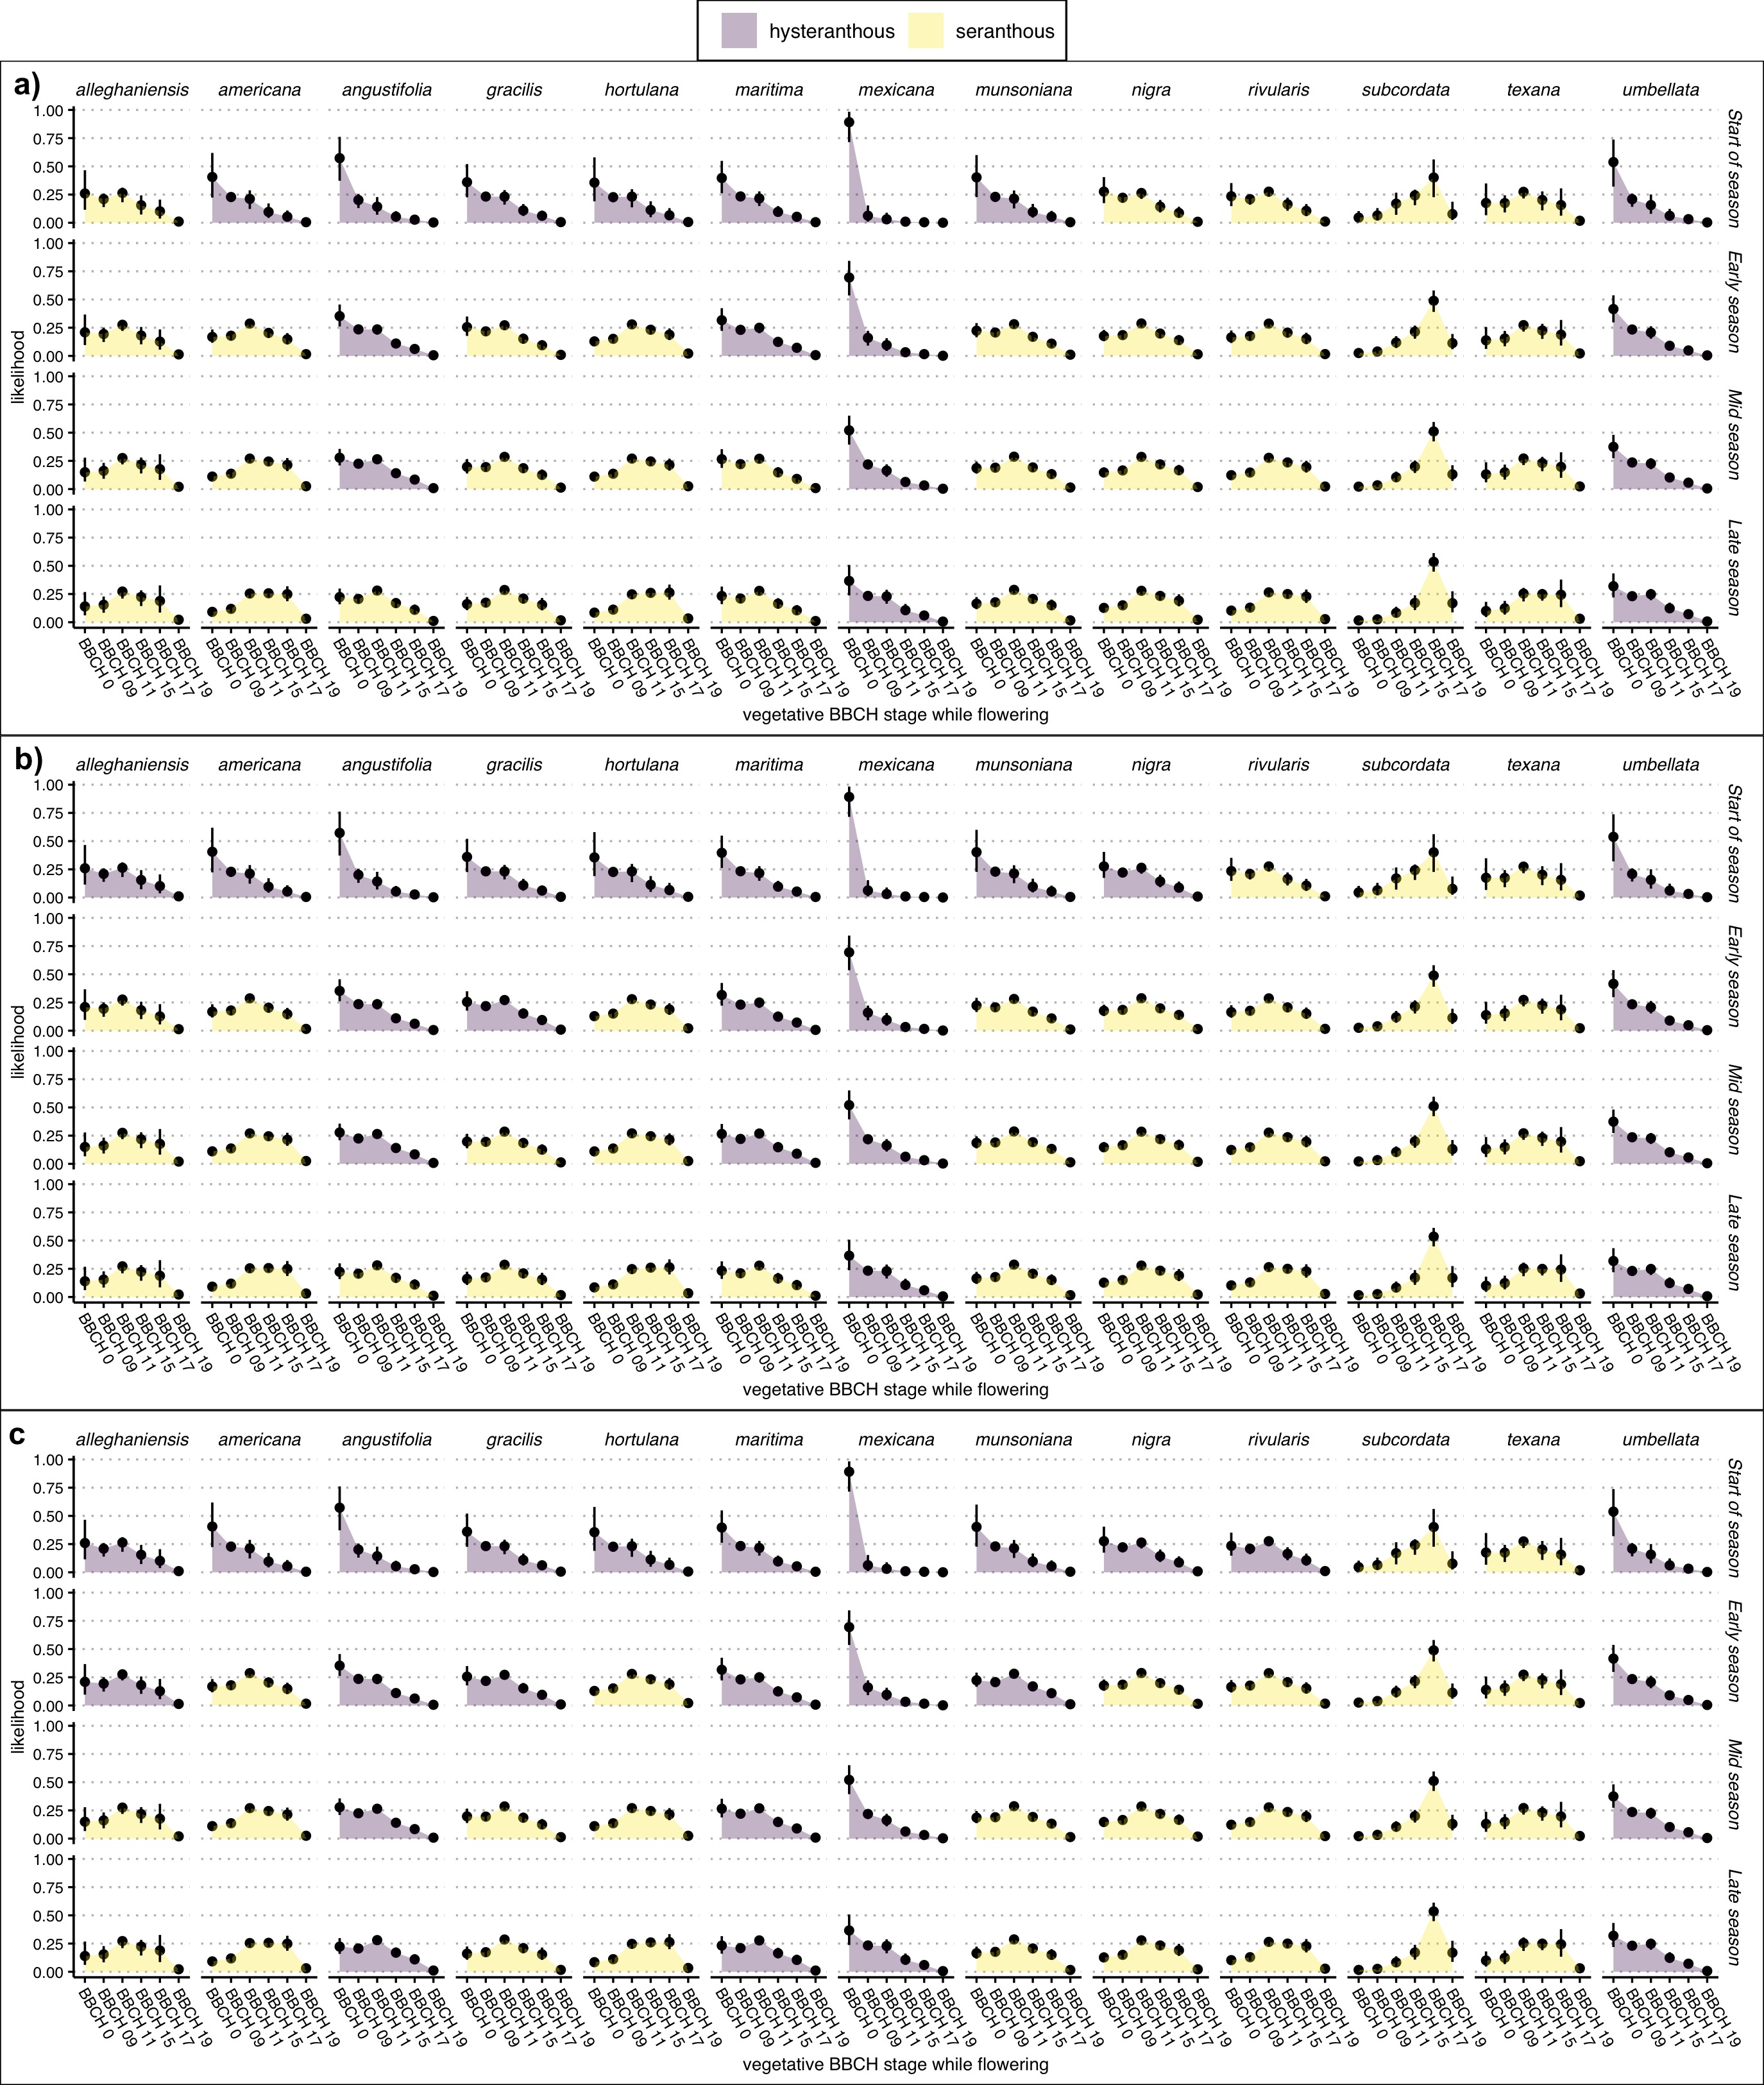
\includegraphics[width=.95\textwidth]{..//..//Plots/ord_quants_phylo.jpeg}
    \caption{Predicted likelihood that a species would be in flower during each vegetative BBCH phase. Points show the mean likelihood while the bar represents the 95\% uncertainty intervals. In a) species were classified as hysteranthous if greater than 50\% probability flowering occurred in BBCH 0 and BBCH 09 (colors) for each part of the flowering season. In b) species were classified as hysteranthous if greater than 25\% probability flowering occurred in BBCH 0 for each part of the flowering season. In c) species were classified as hysteranthous if greater than 40\% probability flowering occurred in BBCH 0 and BBCH 09 for each part of the flowering season.}
    \label{fig:plums}
\end{figure}

\end{document}
